% Template for ICASSP-2010 paper; to be used with:
%          spconf.sty  - ICASSP/ICIP LaTeX style file, and
%          IEEEbib.bst - IEEE bibliography style file.
% --------------------------------------------------------------------------
\documentclass{article}
\usepackage{spconf,amsmath,graphicx}
\usepackage{url}

% Example definitions.
% --------------------
\def\x{{\mathbf x}}
\def\L{{\cal L}}

% Title.
% ------
\title{IMPUTATION OF BEAT-ALIGNED FEATURES AND MUSIC PATTERN LEARNING}
%
% Single address.
% ---------------
%\name{Thierry Bertin-Mahieux\thanks{Thanks to NSERC and some other stuff.}}
%\address{EE dept., Columbia University}
%
% For example:
% ------------
%\address{School\\
%	Department\\
%	Address}
%
% Two addresses (uncomment and modify for two-address case).
% ----------------------------------------------------------
\twoauthors
  {Thierry Bertin-Mahieux\sthanks{TBM is supported in part by a NSERC PG scholarship.}, Ron J. Weiss\sthanks{Thanks something}}
	{Columbia University / New York University\\
          LabROSA / MARL\\
	New York, USA}
  {Graham Grindlay and Daniel P.W. Ellis}
	{Columbia University\\
          LabROSA\\
	New York, USA}

\begin{document}
%\ninept
%
\maketitle
%
\begin{abstract}
Imputation is cool. It is a well-defined problem, as opposed to segmentation.
Gives a reasonable benchmark to compare algorithms that claim learning meaningful
patterns on music. Hard to beat benchmarks comparison, for instance linear
prediction. We compare some methods on a large dataset. We'll track you down
if you don't accept this paper.
\end{abstract}
%
\begin{keywords}
Missing data, chroma features, beat imputation, codebook learning
\end{keywords}
%
\section{Introduction}
\label{sec:intro}
Many signals show similarities and repetitions over time. Learning these repetitions
in an unsupervised way remains a challenge. One reason is the lack of meaningful
tasks to evaluate such learning. Encoding quality serves its purpose, to measure
how faithful a saved or streamd media format is. But having a good encoding
does not mean we understood much about the underlying signal. Denoising is more
interesting as it assumes some knowledge of the media, even if sometimes it relies
solely on local constraints. Needless to say that denoising has been well studied 
for images and speech, among others.

Signals remain where denoising bear little sense, and music is an obvious case.
If the goal is to learn typical harmonic patterns, adding then removing gaussian
noise does not measure the right thing. Imputation of some random frequencies
for some given time $t$ is also oversimplified. Such missing info can usually
be inferred by the restof the information available at time $t$, thus without
using any information over time.

To overcomb these problems, we study here the task of imputing missing information
for full timesteps of music (measured in beats). This is a well-defined task
as the goal is to recover some known masked data. It can easily be evaluated on a
large-scale dataset as music is freely available and the mask can be chosen
at random. It has practical applications, we can imagine the case of streamed music
with some connection problem. Imputing reasonable audio for a few seconds would
be a great alternative to simply stop the stream for a while. Finally, it is a
task that can only be solved by learning meaningful patterns of music over time.

This work should be seen as a first milestone towards solving that task.
After defining it correctly, we try a range of methods to see which ones should
be use as benchmarks in the future. We also look at which algorithms are more robust
to an increasingly larger mask. The code for all the experiments is available
online.

This paper is organized as follow: first we present related work, then we define the
task, including error measures and features used. In Section \ref{sec:methods},
we present the different methods used to tackle imputation, ranging from trivial
to complex. We experiment with these on a common dataset, then conclude in
Section \ref{sec:conclusion} with many avenues of research for future work.

Two writing conventions, we use the terms ``missing'' and ``masked'' interchangeably.
A ``pixel'' is defined as one point of a feature matrix, analoguous to an image.

\section{RELATED WORK}
\label{sec:relatedwork}
Imputation has been studied in many fields, for instance speech 
\cite{Morris1998,Reyes-Gomez2005,Smaragdis2009}, music \cite{Hoffman2010} 
and bioinformatics \cite{Oba2003}.
However, rarely a full slice of time is fully masked (cases $2$ and $3$
in Figure \ref{fig:typeimputation}).

The task of learning the next missing time frame is implicitely studied in recurrent
neural networks as the model is usually trained this way. However, few work deal
with learning more than one missing time frame in advance. Note that recurrent neural
network has been used to learn time aligned beats of music for music composition
\cite{Todd1989,Mozer1994a,Eck2002d}, thus this task has some similarities with our current
work. Another implicitely linked task is modeling music expectation \cite{Hazan2010}, but it deals
with characterizing the upcoming beats of music instead of predicting them.
We will not mention these any further, since the state of the art is difficult to measure.

Imputation should be used to measure the quality of learned patterns. Recent work in 
learning music patterns using features derived from audio include 
\cite{Anglade2009,Bertin-Mahieux2010a,Casey2007,Weiss2010}.

Finally, if the mask span enough beats (i.e. more than one ``music segment''), any good
solution has to deal with music segmentation. Music segmentation based on similar features as
the ones used in this work include \cite{Weiss2010,Levy2008,Mauch2009}.



\section{TASK DEFINITION}
\label{sec:task}

\begin{figure}[t]
\begin{center}
\includegraphics[width=.9\columnwidth]{basic_example}
\end{center}
\caption{Basic example}
\label{fig:code}
\end{figure}

In this work, imputation is defined as recovering a set of adjacent missing beats.
The number of missing beats can vary from $1$ to most of the song. The algorithm
is allowed to use the unmasked part of the song and / or any information learned
on a larger set of songs not including the masked part. This would correspond
to the middle case in Figure \ref{fig:typeimputation}.

In our case, we try to recover chroma features and we never mask the beginning
nor the end of the song, but this is not a absolute constraint of the task.
The long term goal is what we call ``extreme imputation'' where the number of
beats to impute is greatly larger than the known data (bottom case in
Figure \ref{fig:typeimputation}). Trivial methods like taking the average beat
should fail on such a task, and method that succeed:
\begin{enumerate}
\item will learn typical patterns from a large set of songs;
\item will know how to reorganize these patterns so that they are coherent together;
\item will know how to reorganize these patterns so that they match the known
data.
\end{enumerate}
Extreme beat imputation measures the full task of learning and using meaningful
audio patterns.

We use beat-aligned chroma features \cite{Ellis2007a}. 
% DAN, can I steal this from your paper?
Chroma features record the intensity associated with each of
the 12 semitones (e.g. piano keys) within one octave, but all octaves
are folded together.
% **************************************
One can see them as a very coarse and noisy music transcription.
They have been used for segmentation \cite{Weiss2010}, 
chord recognition \cite{Mauch2009} and cover recognition \cite{Ellis2007a}
among others. The specific implementation we use is the one returned
by the Echo Nest API \cite{EchoNest} which uses a constant-Q spectrogram
and where the chroma for each time stamp is normalized so the max is $1$.

The reconstruction error (or divergence) measure is not obvious. In this work,
we report the euclidean distance and the symmetric Kullback-Leibler divergence.
In \cite{Sajda2003}, author discuss the two for
a NMF method and show that they depend on the noise model that is assumed.
A poisson noise model (versus a gaussian one) seems to better fit audio perception, 
which result in the use of KL. See also \cite{Fevotte2009} for a comparison on an
audio excerpt of piano.

We also use absolute normalize difference entropy (ANDE) because it makes us look good, 
we took it from \cite{Mentzelopoulos2004}.
ANDE between two vectors is computed as follow. First, compute the normalized histogram 
of values, in our case we discretize $(0,1)$ in $\mbox{\# bins} = 10$. 
Then, we compute the entropy
$e_b = - log_2 b_b$ of each of the bins $b_{bi}$for each vector $i$. Finally:
\[
\mbox{ANDE} = \left( \Sigma_b \frac{e_{b1} - e_{b2}}{e_{b1}} \right) / (\mbox{\# bins})
\]
Note that ANDE is not symmetric. In our experiment, the first vector is the original one.

\begin{figure}[t]
\begin{center}
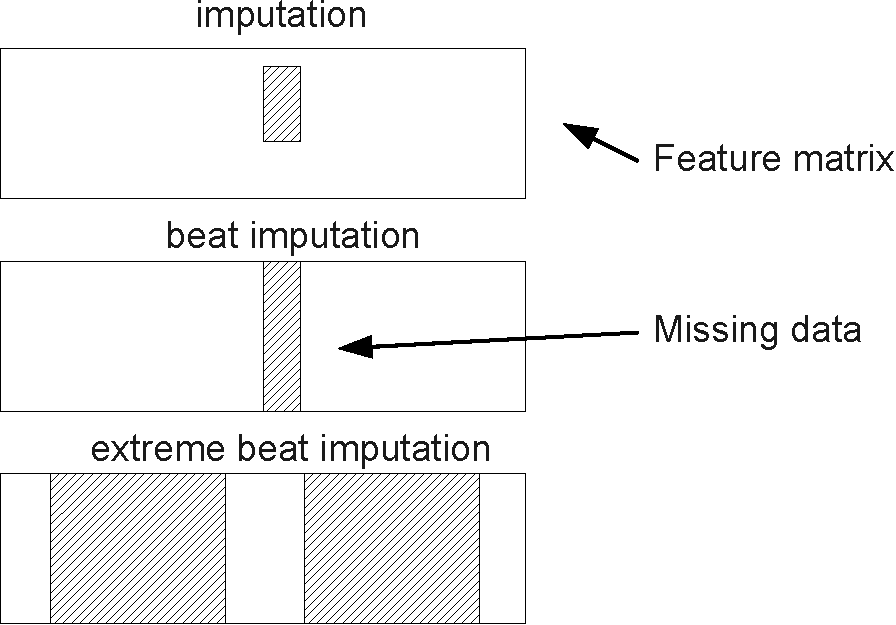
\includegraphics[width=.9\columnwidth]{type_imputation}
\end{center}
\caption{Types of imputation.}
\label{fig:typeimputation}
\end{figure}

\section{METHODS}
\label{sec:methods}
We present the different methods we use for imputing the missing data.
The ``trivial methods'' do not require any learning, and simply use the available
data from the rest of the song to make an educated guess.

The learned models are of more interest for future research, even though they do not
necessarily perform better at the moment. Learning a model that predicts subsequent
notes or harmonic patterns can be applied to other tasks such as cover recognition,
segmentation, similarity and compression.

\subsection{TRIVIAL METHODS}
\label{ssec:trivialmethods}
Below are four of the methods we evaluate, starting by the name we use in the experiments
to refer to them.
\begin{enumerate}
\item \textbf{Random}: each missing pixel is filled with a pseudo-random number drawn from
a constant $[0,1)$ distribution.
\item \textbf{Random-song}: each missing beat is filled with another beat from the song,
chosen at random.
\item \textbf{Average}: each missing beat is filled with the average of the nearby beats,
the window size of nearby beats being a parameter. Note that we look at both previous and
later beats.
\item \textbf{Knn-song}: we compare a window of beats around the missing one with
all possible windows of the same size in the song. We use the closest one (based on euclidean
distance or KL-divergence) to fill in the missing beat. Note that we look at both
previous and later beats.
\end{enumerate}

\subsection{LEARNED MODELS}
\label{ssec:learnedmodels}

Linear predictor, codebook, SIPLCA.

SIPLCA code available online \cite{Weiss2010}. Code to get Echo Nest features and perform
online clustering available online \cite{Bertin-Mahieux2010a}.

HMM \cite{Rabiner1989}.

Imputation is implemented the same way for SIPLCA, Kalman filtering and HMM? Each iteration,
we replace the missing data by the most probable observation according to the model.
For SIPLCA, it is the current reconstruction. For Kalman filtering, it is the most likely
observation based on the current state. This technique has been explored in \cite{Zhang2006}.


\section{EXPERIMENTS}
\label{sec:experiments}
We build beat-align chromagrams using the beat tracking and chroma features as
returned by the Echo Nest API \cite{EchoNest}. Our results are on the Cowbell
dataset (or subset of it) made of $43,000$ songs \cite{Bertin-Mahieux2010a}.

\begin{figure}[t]
\begin{center}
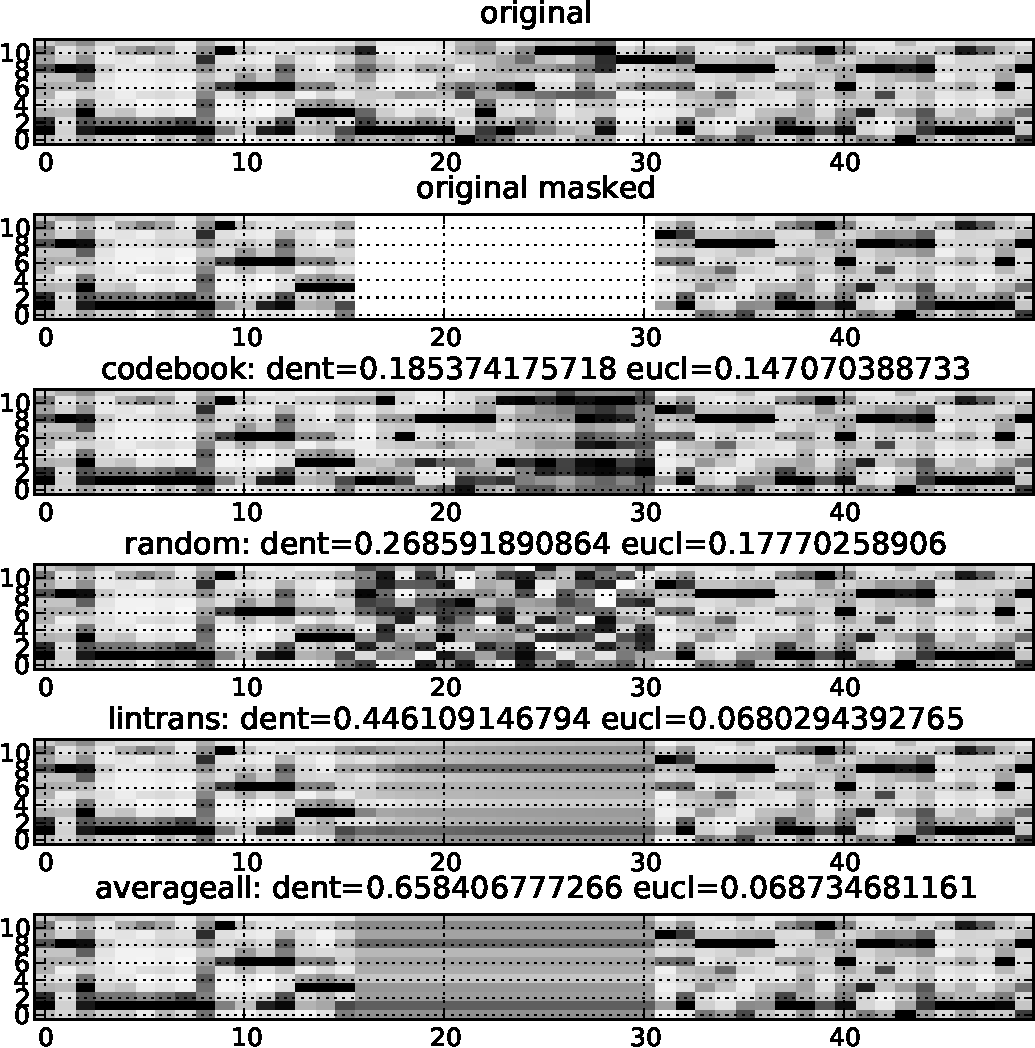
\includegraphics[width=.9\columnwidth]{recon_per_dent}
\end{center}
\caption{Reconstruction of $15$ beats of song by $4$ methods, ordered by
ANDE of the reconstruction. Here ``codebook'' is done with patches of 
size $8$ taken from the visible part of the song. ``dent'' means ANDE,
to be fixed.}
\label{fig:dent}
\end{figure}

Figure \ref{fig:dent} illustrate the use of the ANDE measure. Even if some
reconstruction are worse according to euclidean distance, ANDE gives a feel
of how musical the result looks. An ANDE of $0$ signifies that we have the 
same entropy in the original and the reconstruction segment.

Until we reach perfect reconstruction, we look for reconstruction that do
well on the two measures. Furthermore, it is important to keep similar
performance when the number of masked beat increases. Methods that do
well by learning an average have a rapidly increasing ANDE, as seen in
Figure \ref{fig:2dscore}. We look for methods that stay in the lower left
corner when the number of data to impute increases.

\begin{figure}[t]
\begin{center}
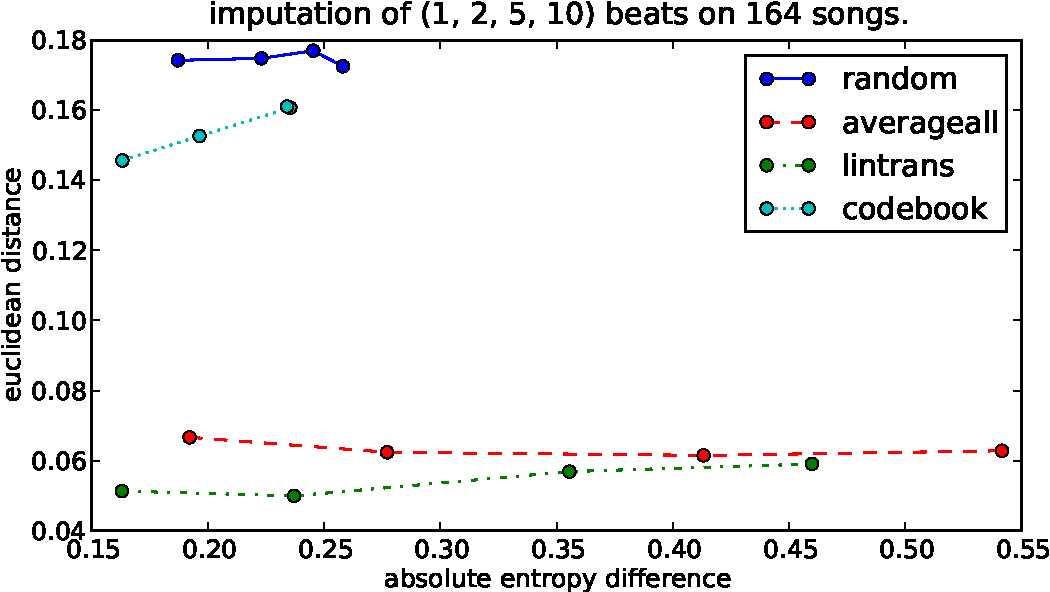
\includegraphics[width=.9\columnwidth]{recon_score_in_2d}
\end{center}
\caption{Reconstruction error for $4$ methods and different
number of masked beats. Errors are ANDE and euclidean
distance. In all cases, the larger the number of masked beats,
the higher the euclidean distance.}
\label{fig:2dscore}
\end{figure}

\begin{figure}[t]
\begin{center}
\includegraphics[width=.9\columnwidth]{imputation}
\end{center}
\caption{Imputation from different methods.}
\label{fig:imputation}
\end{figure}

\begin{table}[t]
\begin{small}
\begin{center}
\begin{tabular}{l|c|c|c|c|c|}
\# beats  & 1 & 2 & 5 & 10 & 15 \\ \hline \hline
random & $0.166$ & $0.166$ & $0.167$ & $0.167$ & $0.168$  \\
rand. song & $0.115$ & $0.114$ & $0.114$ & $0.115$ & $0.115$  \\
average all & $0.057$ & $0.057$ & $0.057$ & $0.057$ & $0.058$ \\
average & $0.047$ & $0.053$ & $0.062$ & $0.065$ & $0.069$ \\ \hline
knn eucl & $0.048$ & $0.049$ & $0.055$ & $0.064$ &  $0.070$ \\
knn kl & $0.049$ & $0.050$ & $0.056$ & $0.066$ &  $0.071$ \\
lin. trans. & $\mathbf{0.044}$ & $\mathbf{0.047}$ & $\mathbf{0.051}$ & $\mathbf{0.053}$ & $\mathbf{0.055}$ \\
codebook & & & & &  \\
SIPLCA & & & & &  \\ \hline
\end{tabular}
\caption{Results based on euclidead distance on $43K$ songs.
Song has to be at least $70$ beats long. 
For ``average'', window is $2$ beats each side of the masked patch.
For ``knn eucl'' and ``knn kl'', window is $10$ beats each side of the masked patch.
For ``lin. trans.'', window is the $2$ previous beats.}
\label{tab:reseucl}
\end{center}
\end{small}
\end{table}

\begin{table}[t]
\begin{small}
\begin{center}
\begin{tabular}{l|c|c|c|c|c|}
\# beats & 1 & 2 & 5 & 10 & 15 \\ \hline \hline
random & $0.428$ & $0.450$ & $0.461$ & $0.461$ & $0.462$  \\
rand. song & $0.334$ & $0.351$ & $0.371$ & $0.377$ & $0.380$  \\
average all & $0.164$ & $0.175$ & $0.183$ & $0.187$ & $0.189$ \\ 
average & $0.121$ & $0.154$ & $0.194$ & $0.212$ &  $0.223$ \\ \hline
knn eucl & $\mathbf{0.116}$ & $0.136$ & $0.169$ & $0.212$ & $0.233$ \\
knn kl & $\mathbf{0.116}$ & $\mathbf{0.135}$ & $\mathbf{0.167}$ & $0.209$ & $0.229$ \\
lin. trans. & $0.141$ & $0.157$ & $0.170$ & $\mathbf{0.180}$ & $\mathbf{0.184}$ \\
codebook & & & & &  \\
SIPLCA & & & & &  \\ \hline
\end{tabular}
\caption{Results based on symmetric KL divergence on $43K$ songs.
See Table \ref{tab:reseucl} for the exact parameters used.}
\label{tab:reskl}
\end{center}
\end{small}
\end{table}

\section{CONCLUSION AND FUTURE WORK}
\label{sec:conclusion}
Push the task as an evaluation for different learning method on such feature.
Way to unify different tasks.

Many algorithms remain to be tried, for instance large scale or deep recurrent
neural network, or using the nonlocal-means algorithm as has been done for
images \cite{Buades2005} and compressive sensing \cite{Gemmeke2008}.
We could boost all those things.

Incorporation of different music-related priors, for instance from chord recognition.

Different kind of masking, e.g. removing only one instrument from the mixture.

Code available at \footnote{Code available at: \url{http://www.columbia.edu/~tb2332/something}}.



% References should be produced using the bibtex program from suitable
% BiBTeX files (here: strings, refs, manuals). The IEEEbib.bst bibliography
% style file from IEEE produces unsorted bibliography list.
% -------------------------------------------------------------------------
\bibliographystyle{IEEEbib}
\bibliography{tbm_bib}

\end{document}
